\subsection{T1: Element-Wise Adaptive Moment and Scalar Control}
\label{sec:t1}

\subsubsection{Family Overview and Meta-Pipeline Position}
\label{sec:t1-overview}


Element-wise adaptive-moment methods are the default optimizer family for
modern Transformer training.  Their defining property is not the mere presence
of momentum, but the preservation of an element-wise update topology: the
optimizer maintains scalar or coordinate-wise state, normalizes or controls
each parameter independently, and avoids exchanging information across rows,
columns, heads, or layers.  T1 therefore contains the Adam-centered adaptive
moment line together with scalar first-order predecessors and outer-control
schemes whose primary mechanism remains element-wise or scalar.  Methods whose
main contribution is matrix routing, irreversible direction discretization,
state compression, or sharpness-aware wrapper gradients are assigned to T2--T5
instead.

\begin{figure*}[t]
  \centering
  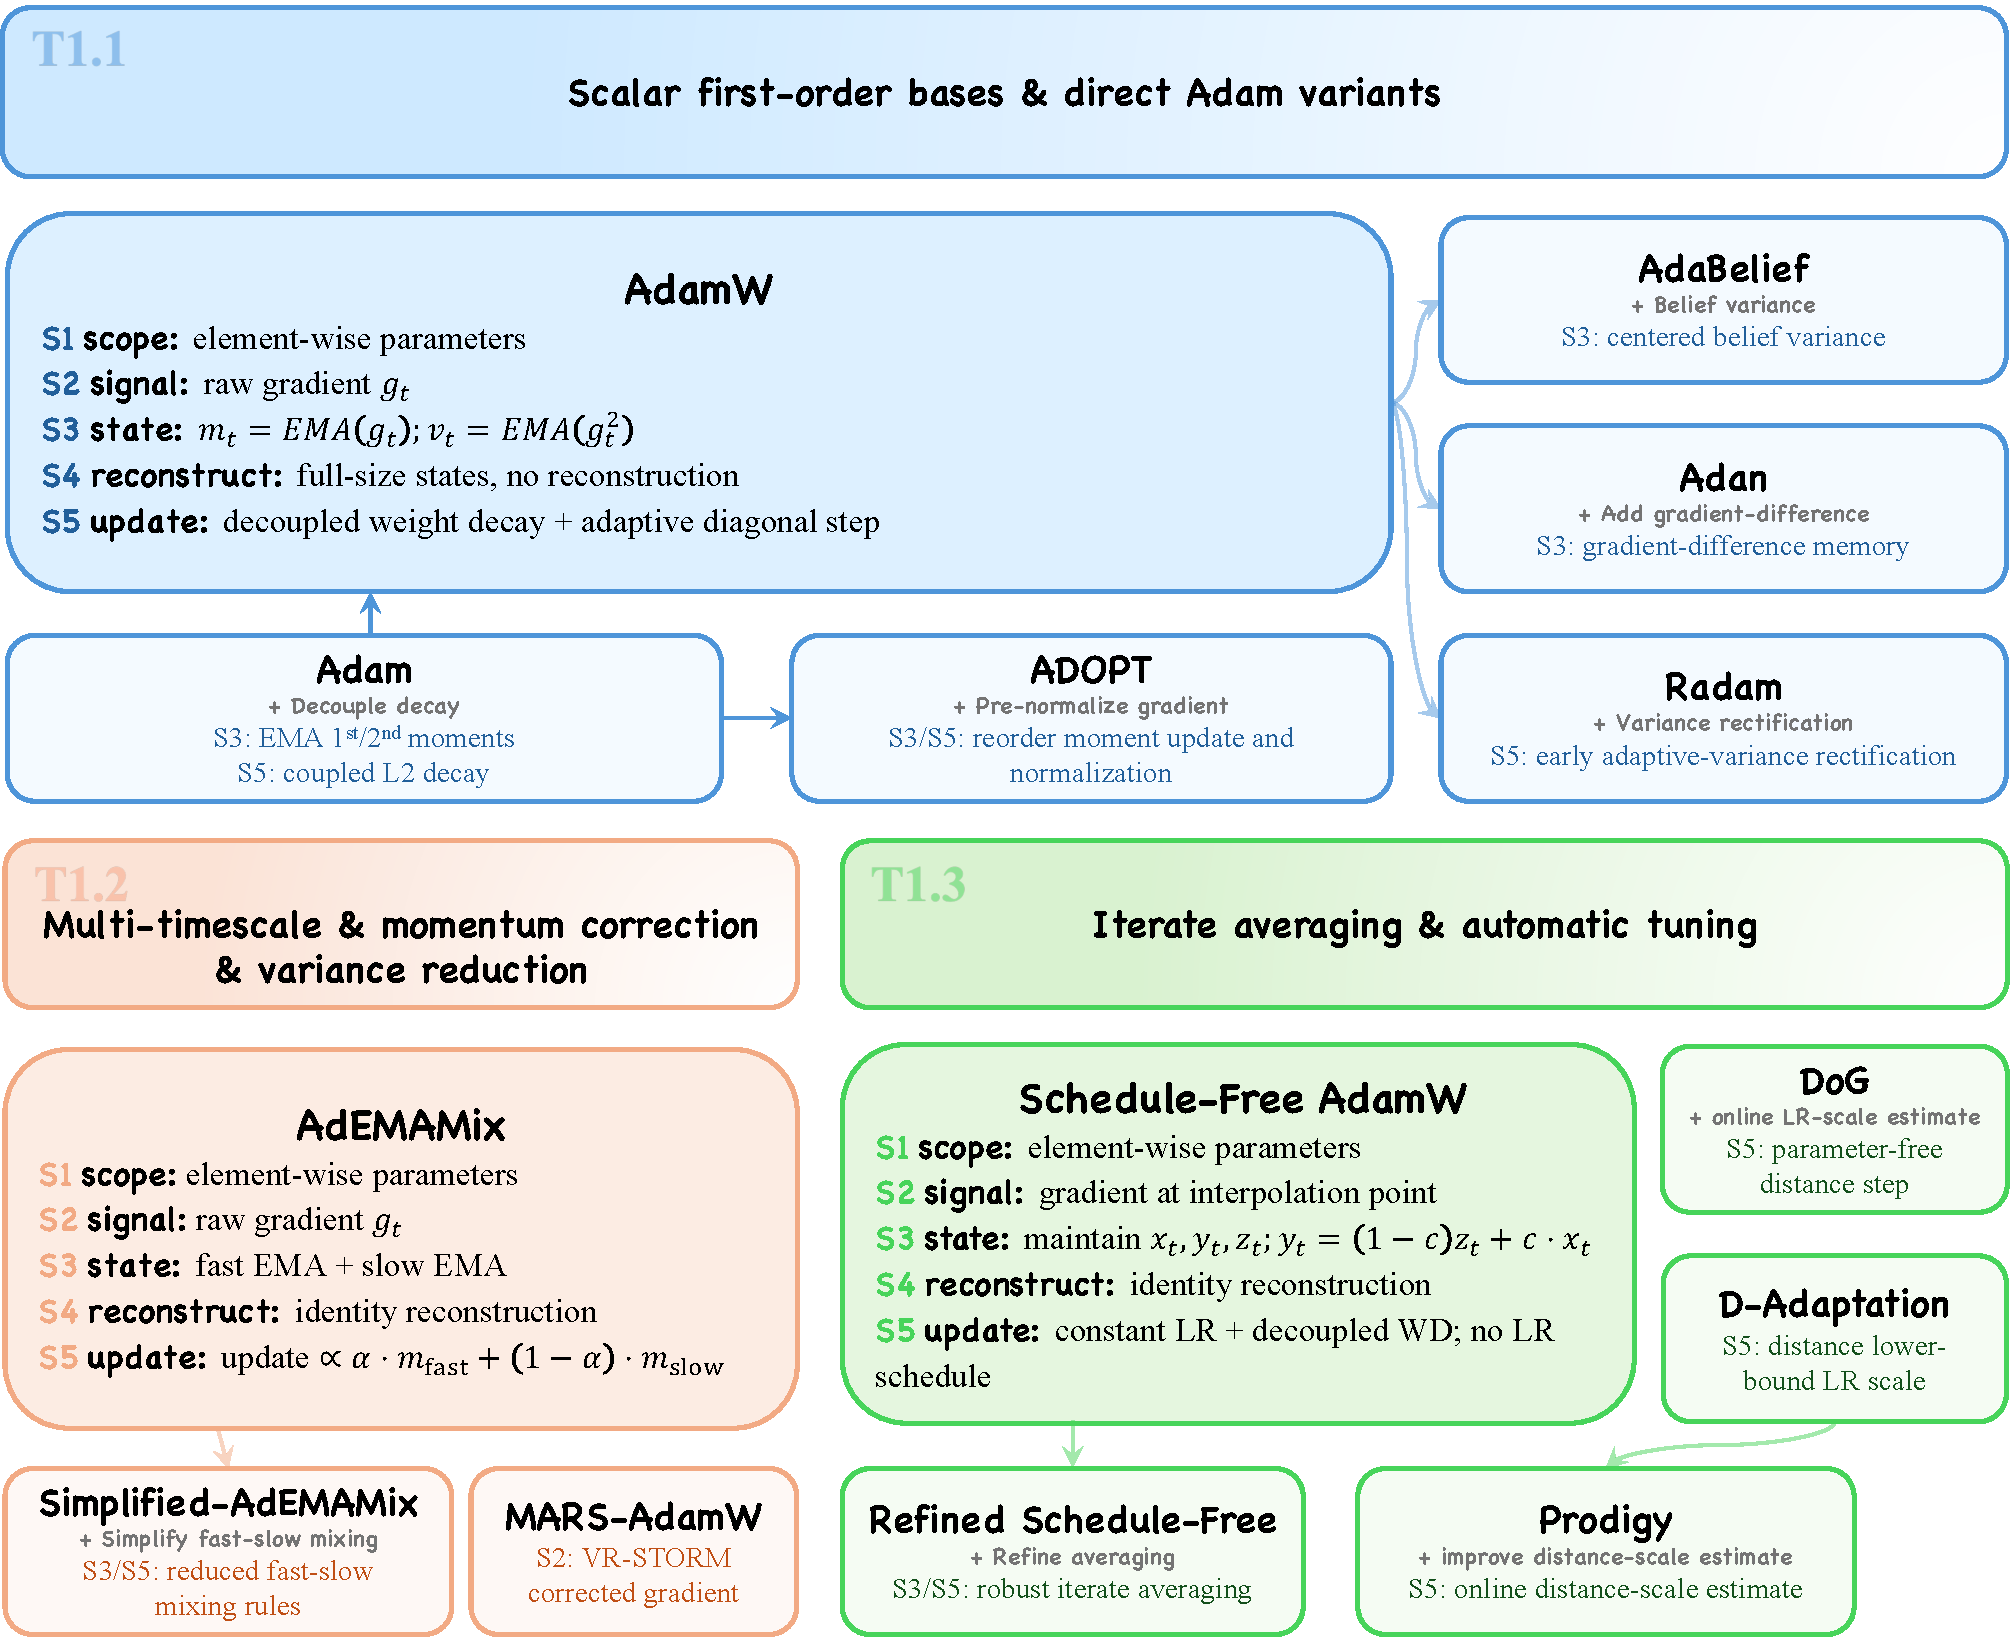
\includegraphics[width=0.75\textwidth]{figures/opt_t1.pdf}
  \caption{Mechanism overview of T1 element-wise adaptive-moment and scalar
  control methods.  The family is organized by the dominant intervention in
  the update: direct scalar or Adam-style variants, additional temporal or
  estimator-correction channels, and outer iterate or global-scale control.
  Boundary methods are shown only when they preserve scalar or element-wise
  update topology.}
  \label{fig:t1_family_mechanism}
\end{figure*}

% Auto-generated by code/generate_taxonomy_figures.py; do not edit by hand.
% \begin{table*}[!htbp]
%   \centering
%   \caption{Taxonomy of element-wise adaptive-moment and scalar-control optimizers.}
%   \label{tab:t1_family_taxonomy}
%   \scriptsize
%   \setlength{\tabcolsep}{4pt}
%   \renewcommand{\arraystretch}{1.16}
%   \arrayrulecolor{optHiddenBlack}
%   \begin{tabularx}{\textwidth}{@{}>{\raggedright\arraybackslash}p{0.27\textwidth}>{\raggedright\arraybackslash}X@{}}
%     \hline
%     \textbf{Subclass} & \textbf{Optimizers} \\
%     \hline
%     \textbf{\textit{T1.1: Scalar First-Order Bases \& Direct Adam Variants}} & Adam~\cite{kingma2015adam}, AdamW~\cite{loshchilov2019decoupled}, NAdam~\cite{dozat2016nadam}, RAdam~\cite{liu2020radam}, Adamax~\cite{kingma2015adam}, AdamX~\cite{tran2019adamx}, Adan~\cite{xie2022adan}, ADOPT~\cite{taniguchi2024adopt}, AdaBelief~\cite{zhuang2020adabelief}, QHAdam~\cite{ma2019qhadam}, DiffGrad~\cite{dubey2019diffgrad}, AdaSmooth~\cite{lu2023adasmooth}, AccSGD~\cite{kidambi2018insufficiency}, AdamD~\cite{john2021adamd}, AdamC~\cite{defazio2025gradients}, AdaBound~\cite{luo2019adabound}, PID~\cite{an2018pid}, AdaMod~\cite{ding2019adamod}, PAdam~\cite{chen2018padam}, EXAdam~\cite{adly2024exadam}, Gravity~\cite{bahrami2021gravity}, VSGD~\cite{schaul2013nomore}, SGDM~\cite{polyak1964some,sutskever2013importance}, AdaGrad~\cite{duchi2011adaptive}, RMSProp~\cite{tieleman2012rmsprop}, AdaDelta~\cite{zeiler2012adadelta} \\
%     \hline
%     \textbf{\textit{T1.2: Multi-Timescale, Momentum Correction \& Variance Reduction}} & AdEMAMix~\cite{pagliardini2024ademamix}, Simplified-AdEMAMix~\cite{morwani2025connections}, MARS~\cite{yuan2024mars}, MARS-AdamW~\cite{yuan2024mars,loshchilov2019decoupled}, MADGRAD~\cite{defazio2022madgrad}, AggMo~\cite{lucas2018aggmo}, MSVAG~\cite{balles2018dissecting}, TAM~\cite{malviya2024torque}, Ranger~\cite{zhang2019lookahead,wright2021ranger21}, Ranger21~\cite{wright2021ranger21} \\
%     \hline
%     \textbf{\textit{T1.3: Iterate Averaging \& Automatic Tuning}} & Schedule-Free AdamW~\cite{defazio2024road,loshchilov2019decoupled}, Schedule-Free SGD~\cite{defazio2024road}, Refined Schedule-Free~\cite{morwani2025connections,song2026through}, Prodigy~\cite{mishchenko2023prodigy}, D-Adaptation~\cite{defazio2023dadaptation}, DoG~\cite{ivgi2023dog}, DoWG~\cite{khaled2023dowg}, SWATS~\cite{keskar2017swats}, SGD-SaI~\cite{xu2024no}, Ali-G~\cite{berrada2020training} \\
%     \hline
%   \end{tabularx}
% \end{table*}

\definecolor{hidden-blue}{HTML}{4a90e2}
\definecolor{hidden-black}{HTML}{333333}
\tikzstyle{my-box}=[
  rectangle,
  draw=hidden-black,
  rounded corners,
  text opacity=1,
  minimum height=1.5em,
  minimum width=5em,
  inner sep=2pt,
  align=center,
  fill opacity=.5,
]
\tikzstyle{root}=[
  align=center,
]
\tikzstyle{leaf}=[
  my-box,
  minimum height=1.5em,
  text=black,
  font=\normalsize,
  inner xsep=5pt,
  inner ysep=4pt,
  text width=10.5em,
  fill opacity=1,
]
\tikzstyle{leaf1}=[
  my-box,
  minimum height=1.5em,
  fill=yellow!32,
  text=black,
  font=\normalsize,
  inner xsep=5pt,
  inner ysep=4pt,
  text width=17em,
  align=left,
]
\tikzstyle{leaf2}=[
  my-box,
  minimum height=1.5em,
  fill=hidden-blue!57,
  text=black,
  font=\normalsize,
  inner xsep=5pt,
  inner ysep=4pt,
  text width=17em,
  align=left,
]
\tikzstyle{leaf3}=[
  my-box,
  minimum height=1.5em,
  fill=purple!27,
  text=black,
  font=\normalsize,
  inner xsep=5pt,
  inner ysep=4pt,
  text width=17em,
  align=left,
]

\begin{figure*}[!htbp]
\centering
\resizebox{\textwidth}{!}{
\begin{forest}
forked edges,
for tree={
grow=east,
reversed=true,
anchor=base west,
parent anchor=east,
child anchor=west,
base=left,
font=\large,
rectangle,
draw=hidden-black,
rounded corners,
align=left,
minimum width=4em,
edge+={darkgray, line width=1pt},
s sep=4pt,
inner xsep=5pt,
inner ysep=4pt,
line width=1.1pt,
ver/.style={rotate=90, child anchor=north, parent anchor=south, anchor=center},
},
where level=1{text width=11em, font=\normalsize}{},
where level=2{text width=34.5em, tier=citations, font=\small}{},
[
    T1-based Optimizers,
    % ver, fill=gray!70, text=white, root
    ver, fill=brown!10!white, text=hidden-black, root
    [
        T1.1: Scalar Bases \& Direct \\ Adam Variants,
        fill=yellow!32, leaf1
        [{
            Adam~\cite{kingma2015adam},
            AdamW~\cite{loshchilov2019decoupled},
            NAdam~\cite{dozat2016nadam},
            RAdam~\cite{liu2020radam},
            Adamax~\cite{kingma2015adam}, \\
            Adan~\cite{xie2022adan},
            ADOPT~\cite{taniguchi2024adopt},
            AdaBelief~\cite{zhuang2020adabelief},
            QHAdam~\cite{ma2019qhadam},
            DiffGrad~\cite{dubey2019diffgrad},
            AccSGD~\cite{kidambi2018insufficiency}, \\
            AdaSmooth~\cite{lu2023adasmooth},
            AdamD~\cite{john2021adamd},
            AdamC~\cite{defazio2025gradients},
            AdaBound~\cite{luo2019adabound},
            PID~\cite{an2018pid},
            AdaMod~\cite{ding2019adamod}, \\
            PAdam~\cite{chen2018padam},
            EXAdam~\cite{adly2024exadam},
            Gravity~\cite{bahrami2021gravity},
            VSGD~\cite{schaul2013nomore},
            SGDM~\cite{polyak1964some,sutskever2013importance},
            AdaGrad~\cite{duchi2011adaptive}, \\
            RMSProp~\cite{tieleman2012rmsprop},
            AdaDelta~\cite{zeiler2012adadelta}
        }, fill=yellow!12]
    ]
    [
        T1.2: Multi-Timescale \& Momentum \\ Correction \& Variance Reduction,
        fill=hidden-blue!57, leaf2
        [{
            AdEMAMix~\cite{pagliardini2024ademamix},
            Simplified-AdEMAMix~\cite{morwani2025connections},
            MARS~\cite{yuan2024mars},
            MARS-AdamW~\cite{yuan2024mars}, \\MADGRAD~\cite{defazio2022madgrad},
            AggMo~\cite{lucas2018aggmo},
            MSVAG~\cite{balles2018dissecting},
            TAM~\cite{malviya2024torque},
            Ranger~\cite{zhang2019lookahead,wright2021ranger21}, \\
            Ranger21~\cite{wright2021ranger21}
        }, fill=hidden-blue!15]
    ]
    [
        T1.3: Iterate Averaging \& Automatic \\ Tuning,
        fill=purple!27, leaf3
        [{
            Schedule-Free AdamW~\cite{defazio2024road,loshchilov2019decoupled},
            Schedule-Free SGD~\cite{defazio2024road},
            DoG~\cite{ivgi2023dog},
            Prodigy~\cite{mishchenko2023prodigy}, \\
            D-Adaptation~\cite{defazio2023dadaptation},
            DoWG~\cite{khaled2023dowg},
            SWATS~\cite{keskar2017swats},
            SGD-SaI~\cite{xu2024no},
            Ali-G~\cite{berrada2020training}, \\
            Refined Schedule-Free~\cite{morwani2025connections,song2026through}
        }, fill=purple!12]
    ]
  ]
\end{forest}
}
\caption{Taxonomy of element-wise adaptive-moment and scalar-control optimizers.}
\label{tab:t1_family_taxonomy}
\end{figure*}

\paragraph{Subclass structure.}
Figure~\ref{tab:t1_family_taxonomy} gives the complete optimizer membership for
T1.  The three subclasses below are therefore used to interpret the taxonomy
figure, rather than to repeat its entries.  The split is mechanism-based
rather than chronological: each subclass identifies the dominant non-identity
operation added around the AdamW coordinate-wise template.
\begin{enumerate}[label=\textbf{T1.\arabic*},leftmargin=*,itemsep=2pt]
  \item \textbf{Scalar bases and direct Adam variants.}
  This subclass groups optimizers whose main change remains local to the
  coordinate-wise template: the numerator, diagonal scale, bias correction,
  decay finalization, or scalar control law.  It includes both the AdamW line
  and historical scalar or diagonal predecessors, but the latter are used as
  conceptual anchors rather than as evidence that all T1 methods are modern
  large-model optimizers.
  \item \textbf{Multi-timescale, momentum correction, and variance reduction.}
  This subclass changes the signal that enters state evolution.  Its members
  add fast/slow temporal channels, replace the raw mini-batch gradient with a
  corrected or variance-reduced estimator, gate momentum by temporal
  alignment, or bundle such components around an Adam or RAdam core.
  \item \textbf{Iterate averaging and automatic tuning.}
  This subclass leaves the scalar or element-wise base update largely intact
  and instead modifies the outer control system: iterate averaging, global
  learning-rate scale inference, initialization-time scaling, or
  optimizer-phase switching.
\end{enumerate}

For a parameter vector
$\theta_t \in \mathbb{R}^d$ and stochastic gradient $g_t$, the canonical
AdamW update maintains
\begin{align}
  m_t &= \beta_1 m_{t-1} + (1-\beta_1) g_t, \quad v_t = \beta_2 v_{t-1} + (1-\beta_2) g_t \odot g_t, \\
  u_t &= \frac{\hat{m}_t}{\sqrt{\hat{v}_t}+\epsilon}, \quad
  \theta_{t+1} = (1-\eta_t \lambda)\theta_t - \eta_t u_t,
  \label{eq:t1-adamw-template}
\end{align}
where hats denote bias correction and weight decay is decoupled from the
adaptive direction~\citep{kingma2015adam,loshchilov2019decoupled}.  The update
constructs a diagonal preconditioner from the second-moment state and leaves
the parameter topology unchanged.  This coordinate-wise invariance is the
central commonality of T1: individual methods may change the numerator, the
variance proxy, bias correction, decay finalization, temporal state, averaged
iterate, or global step-size scale, but they do not introduce matrix-level
basis changes, low-rank reconstruction, quantized state representation, or
sharpness-aware auxiliary gradients.  Scalar-control boundary methods can be
viewed as setting the adaptive denominator to an identity scale, while
historical adaptive-rate methods provide the diagonal-statistics lineage from
which Adam-style updates emerged.

In the meta-pipeline of Section~\ref{sec:meta-pipeline}, T1 is mostly
identity-like in S1, S2, and S4.  Parameters are routed at their native
coordinate granularity (S1), the stochastic gradient is usually passed directly
into the update rule (S2), and the reconstructed update remains
full-dimensional (S4).  The primary non-identity operation is S3 state
evolution: the optimizer specifies which moving averages, variance proxies,
time scales, cross-moment corrections, variance-reduced estimators, or
averaged iterates are maintained.  S5 supplies the second locus of variation:
AdamW decouples weight decay, RAdam rectifies early adaptive variance, AdamC
adjusts decay--schedule interactions, D-Adaptation and Prodigy infer a global
learning-rate scale, and Schedule-Free methods internalize the role of an
external learning-rate schedule through iterate averaging.

\subsubsection{LMO-Driven Four-Axis Interpretation}
\label{sec:t1-lmo-four-axis}

In the four-axis view, the common T1 coordinate is
\begin{equation}
  \big((I,I),\ \psi,\ \hat{H}_t,\ \alpha,\ \widehat{g}_t,\ \mathrm{Full}\big),
\end{equation}
where the analysis basis is the identity, the curvature estimate is diagonal,
and the state is stored at full coordinate resolution.  AdamW corresponds to
$\hat{H}_t=\operatorname{diag}(\hat{v}_t)$ and
$\alpha=\tfrac{1}{2}$, yielding the square-root preconditioned direction in
Eq.~\eqref{eq:t1-adamw-template}.  Under the Fisher identity discussed in
Section~\ref{sec:prelim-background}, the EMA of $g_t \odot g_t$ can be read as
a diagonal Fisher or Gauss--Newton surrogate.  This makes the family a
diagonal-curvature analogue of the matrix preconditioners in T2, but with no
off-diagonal coupling and no basis change.

The LMO interpretation clarifies what is shared and what is not shared across
T1.  If the adaptive denominator is temporarily fixed, the numerator selects a
coordinate-wise descent pattern.  In the limiting normalized view, a signed
coordinate direction is the LMO solution over an $\ell_\infty$-type ball, and
the diagonal denominator deforms that ball into an anisotropic, coordinate-wise
trust region.  AdamW should therefore not be reduced to either ``sign descent''
or ``Newton descent.''  Its practical update combines an element-wise
directional component, a diagonal curvature scale, bias correction, damping,
and a global step-size schedule.  This is why T1 methods often share the same
Axis~I basis and Axis~III exponent while differing mainly in Axis~II
curvature/variance estimation and gradient-estimation quality, and S5
step-size or regularization control.  Boundary methods with no adaptive
denominator can be viewed as using $\hat{H}_t=I$ and $\alpha=0$; they are
kept in T1 only as scalar first-order predecessors or control schemes, not as
evidence that every T1 method is an adaptive-moment estimator.

This view also separates T1 from neighboring families.  Lion belongs to T3
because its defining operation is an irreversible sign map and it removes the
second-moment state, even though it inherits an Adam-like momentum
interface~\citep{chen2023symbolic}.  AdaFactor belongs to T4 because its
defining contribution is factorized storage of the second-moment state, not a
new full-state moment estimator.  Sophia belongs to T5 because it replaces the
Adam variance proxy with an explicit curvature estimate and clipped
trust-region update~\citep{liu2023sophia}.  T1 is therefore the baseline
coordinate system from which many later optimizers depart.

\subsubsection{Representative Methods}
\label{sec:t1-methods}

Against the subclass map above, the representative methods are organized by
three recurring mechanism patterns: local modifications of AdamW's numerator,
denominator, bias correction, or writeback; additional temporal or
variance-reduced signals; and outer rules for averaging, global scale
inference, or switching.

\paragraph{Scalar Bases and Direct Adam Variants.}
\label{sec:t1-standard-variants}

The first branch is the broadest part of T1.  Its members are best read in
tiers, because some are historical scalar bases, some define the modern Adam
baseline, and some are local corrections to one term of the AdamW template:
at the survey level, they can be summarized as
\begin{equation}
  u_t = \frac{a_t}{b_t+\epsilon}, \quad
  \theta_{t+1} = \theta_t - \eta_t u_t - \eta_t \lambda_t \chi_t(\theta_t),
  \label{eq:t1-direct-variant-template}
\end{equation}
where $a_t$ is a momentum-like numerator, $b_t$ is a diagonal scale or
variance proxy, and $\chi_t$ specifies whether decay is coupled to the
gradient channel or decoupled at writeback.
\begin{itemize}
  \setlength{\itemsep}{2pt}
  \item \textbf{Scalar and diagonal predecessors.}  SGDM introduced a
  heavy-ball momentum buffer for smoother descent
  ~\citep{polyak1964some,sutskever2013importance}; AdaGrad accumulated squared
  gradients to produce coordinate-wise learning rates~\citep{duchi2011adaptive};
  RMSProp replaced AdaGrad's cumulative sum with a running average
  ~\citep{tieleman2012rmsprop}; AdaDelta used ratios of running RMS quantities
  to reduce manual learning-rate dependence~\citep{zeiler2012adadelta}; and
  VSGD estimated local gradient statistics to adapt learning rates
  ~\citep{schaul2013nomore}.  These methods are not all Adam-like, but they
  form the scalar and diagonal-control substrate from which Adam-style methods
  developed.
  \item \textbf{Adam baseline line.}  Adam combined first-moment momentum,
  RMSProp-style second moments, and bias correction into a single adaptive
  method~\citep{kingma2015adam}; Adamax replaces the second-moment denominator
  with an exponentially weighted $\ell_\infty$ norm; and AdamW became the
  practical large-model baseline by decoupling weight decay from the adaptive
  gradient normalizer~\citep{loshchilov2019decoupled}.  In the meta-pipeline,
  AdamW is mainly an S5 change: the direction $u_t$ is computed as in Adam,
  while shrinkage is applied directly to parameters rather than being mixed
  into $g_t$.
  \item \textbf{High-salience direct Adam variants.}  NAdam inserts a
  Nesterov-style lookahead term into Adam's first-moment pathway
  ~\citep{dozat2016nadam}.  RAdam adds a rectification factor for the
  high-variance early adaptive denominator~\citep{liu2020radam}.  AdaBelief
  replaces $g_t^2$ with the centered prediction-error statistic $(g_t-m_t)^2$
  ~\citep{zhuang2020adabelief}.  Adan adds a Nesterov-inspired
  gradient-difference channel using both $g_t$ and $g_t-g_{t-1}$
  ~\citep{xie2022adan}.  ADOPT changes the ordering of second-moment update and
  normalization to obtain guarantees for arbitrary $\beta_2$
  ~\citep{taniguchi2024adopt}.  EXAdam adds adaptive cross-moment debiasing and
  gradient-based acceleration while remaining a direct Adam extension
  ~\citep{adly2024exadam}.
  \item \textbf{Local adaptivity and correction variants.}  QHAdam interpolates
  between immediate and momentum-based directions through quasi-hyperbolic
  weighting~\citep{ma2019qhadam}; AdaMod bounds Adam's adaptive learning rates
  using a momental upper bound~\citep{ding2019adamod}; and PAdam interpolates
  between Adam (or AMSGrad) and SGDM through a partial-adaptivity exponent
  ~\citep{chen2018padam}.  DiffGrad and AdaSmooth adapt learning rates from
  gradient-change or effective-ratio signals
  ~\citep{dubey2019diffgrad,lu2023adasmooth}; AdamD modifies bias correction
  ~\citep{john2021adamd}; and AdamC corrects decay--schedule interactions near
  the end of long-duration training~\citep{defazio2025gradients}.
  \item \textbf{Boundary scalar-control methods.}  AccSGD, PID, and Gravity
  remain in T1.1 only as scalar-control boundary cases
  ~\citep{kidambi2018insufficiency,an2018pid,bahrami2021gravity}.  They help
  explain the control-theoretic and acceleration background of the family, but
  they should not receive the same narrative weight as AdamW, RAdam, AdaBelief,
  Adan, or ADOPT when the target setting is modern LLM training.
\end{itemize}

This tiered reading prevents T1.1 from becoming a flat list of names.  The
central comparison is AdamW versus direct modifications of AdamW's numerator,
denominator, bias correction, or writeback rule; the historical and boundary
methods provide context and ablation anchors.  Several direct variants can be
viewed as substitutions inside Eq.~\eqref{eq:t1-direct-variant-template}; for
example,
\begin{align}
  v_t^{\mathrm{Belief}}
    &= \beta_2 v_{t-1}^{\mathrm{Belief}}
       + (1-\beta_2)(g_t-m_t)\odot(g_t-m_t), \\
  u_t^{\mathrm{RAdam}}
    &= r_t \frac{\hat{m}_t}{\sqrt{\hat{v}_t}+\epsilon}, \quad
  u_t^{\mathrm{PAdam}}
    = \frac{\hat{m}_t}{(\hat{v}_t)^p+\epsilon}.
  \label{eq:t1-direct-substitutions}
\end{align}
These formulas do not make AdaBelief, RAdam, and PAdam the same method; they
show that their primary changes remain local to the diagonal variance proxy,
early-step rectification, or adaptivity exponent.

\paragraph{Multi-Timescale, Momentum Correction, and Variance Reduction.}
\label{sec:t1-multitimescale}

The second branch asks whether a single raw EMA stream is enough.  A fast
momentum reacts to the current mini-batch distribution but is noisy; a slow
momentum is stable but can lag behind regime changes; and a variance-reduced
or alignment-corrected signal can change the quality of the gradient entering
state evolution.  We therefore separate the branch into four mechanism groups:
\begin{equation}
  \widehat{g}_t = \mathcal{C}_t(g_t,g_{t-1},m_{t-1}), \quad
  m_t^{(k)} = \beta_k m_{t-1}^{(k)} + (1-\beta_k)\widehat{g}_t,\quad
  a_t = \sum_{k=1}^{K}\omega_k m_t^{(k)}.
  \label{eq:t1-temporal-template}
\end{equation}
Here $\mathcal{C}_t$ denotes a possible estimator correction and the
$m_t^{(k)}$ streams denote different temporal channels.  Standard AdamW is
the special case $K=1$ and $\widehat{g}_t=g_t$.
\begin{itemize}
  \setlength{\itemsep}{2pt}
  \item \textbf{Multi-time-scale momentum.}  AdEMAMix maintains both a standard
  fast EMA and an older, slower EMA, then mixes them in the update direction
  ~\citep{pagliardini2024ademamix}.  This is especially relevant to LLM
  training, where long horizons can make old gradient information useful
  rather than stale.  Simplified-AdEMAMix preserves the interpretation while
  exposing connections to schedule-free and accelerated SGD variants
  ~\citep{morwani2025connections}.  AggMo is the earlier multi-time-scale
  analogue, aggregating several momentum buffers with different decay rates
  ~\citep{lucas2018aggmo}.
  \item \textbf{Variance-reduced or corrected estimators.}  MARS introduces a
  scaled stochastic recursive momentum estimator that can be paired with AdamW,
  Lion, or Shampoo-style bases~\citep{yuan2024mars}.  In the AdamW instance,
  the signal entering S3 is no longer raw $g_t$ but a gradient-difference
  corrected estimator, so the method changes Axis~II while preserving the
  element-wise base update.  MADGRAD combines AdaGrad-style accumulated
  curvature with a momentumized dual-averaged update~\citep{defazio2022madgrad}.
  MSVAG is more diagnostic than deployment driven: it decomposes Adam into
  sign, magnitude, and variance effects~\citep{balles2018dissecting}.
  \item \textbf{Alignment-aware momentum correction.}  TAM is neither a
  multi-time-scale method nor a STORM-style variance-reduction method.  It
  damps momentum injection according to the alignment between current gradients
  and historical momentum~\citep{malviya2024torque}.  Its role in T1.2 is to show
  that momentum can be corrected by geometry of temporal agreement, not only
  by adding an older EMA or recursive estimator.
  \item \textbf{Composite optimizer bundles.}  Ranger combines RAdam,
  Lookahead, and often gradient centralization; Ranger21 combines AdamW with a
  larger set of stabilization components
  ~\citep{zhang2019lookahead,wright2021ranger21}.  These methods are useful
  implementation bundles, but their components occupy different meta-pipeline
  slots.  We keep them connected to T1 through their Adam or RAdam core and record
  Lookahead-style averaging or post-processing as secondary tags.
\end{itemize}

The common thread is that T1.2 no longer trusts one raw momentum stream as the
only temporal signal.  It either adds more time scales, corrects the estimator
fed into S3, or gates momentum by temporal alignment while leaving routing and
writeback largely element-wise.  In this notation, AdEMAMix primarily changes
$K$ and $\omega_k$; MARS changes $\mathcal{C}_t$ before the AdamW-like state
update; and TAM can be read as inserting an alignment-dependent gate, e.g.,
\begin{equation}
  \widehat{g}_t = \kappa_t g_t, \quad
  \kappa_t = f\!\left(
    \frac{\langle g_t,m_{t-1}\rangle}
         {\|g_t\|\,\|m_{t-1}\|+\epsilon}
  \right),
  \label{eq:t1-alignment-gate}
\end{equation}
where Eq.~\eqref{eq:t1-alignment-gate} is a template for the class of
alignment-aware corrections rather than a replacement for the exact algorithm
in each paper.

\paragraph{Iterate Averaging and Automatic Tuning.}
\label{sec:t1-averaging-autotuning}

The third branch does not primarily change the coordinate-wise denominator.
Instead, it changes the outer control logic around a scalar or element-wise
base optimizer: how iterates are averaged, how the global scale is chosen, or
when the optimizer should change phase.  The subclass has three readable
groups:
\begin{equation}
  y_t = (1-\rho_t)x_t+\rho_t \bar{x}_t, \quad
  x_{t+1}=x_t-\eta_t u_t(y_t), \quad
  \eta_t=\eta_{\mathrm{base}}\,d_t,
  \label{eq:t1-outer-control-template}
\end{equation}
where $y_t$ is an interpolation point, $\bar{x}_t$ is an averaged iterate, and
$d_t$ is an inferred global scale.  Schedule-free methods emphasize the first
two terms; learning-rate-free methods emphasize the online construction of
$d_t$; switching methods change which base rule defines $u_t$.
\begin{itemize}
  \setlength{\itemsep}{2pt}
  \item \textbf{Schedule-free iterate systems.}  Schedule-Free optimization
  replaces an externally prescribed learning-rate schedule with an internal
  iterate-averaging mechanism~\citep{defazio2024road}.  In the AdamW instance,
  the optimizer maintains training, evaluation, and averaged iterates, evaluates
  gradients at an interpolation point, and uses a constant learning-rate
  interface with decoupled weight decay.  Refined Schedule-Free methods further
  analyze language-model trajectories and adjust the method for robustness to
  momentum and large-batch settings~\citep{song2026through}.  Schedule-Free SGD
  is kept in the same subclass as the scalar-base analogue.
  \item \textbf{Learning-rate-free scale inference.}  D-Adaptation estimates a
  lower bound on the distance to the solution online and uses it to set the
  learning-rate scale without line search or extra gradient evaluations
  ~\citep{defazio2023dadaptation}.  Prodigy estimates the same distance scale
  more aggressively and can be used with Adam-like adaptive methods
  ~\citep{mishchenko2023prodigy}.  DoG and DoWG form a related
  parameter-free path, setting dynamic step sizes from distance-over-gradient
  quantities rather than a user-specified learning rate
  ~\citep{ivgi2023dog,khaled2023dowg}.
  \item \textbf{Switching, initialization-time scaling, and global clipping.}
  SWATS starts with Adam and switches to SGD when an estimated SGD learning
  rate becomes stable, aiming to combine Adam's fast early progress with
  SGD-like later generalization~\citep{keskar2017swats}.  SGD-SaI avoids
  Adam-like second-moment state during training and uses an initialization-time
  group signal-to-noise estimate to set learning-rate scales
  ~\citep{xu2024no}.  Ali-G computes adaptive global learning rates
  from interpolation assumptions and clipping~\citep{berrada2020training}.
\end{itemize}

T1.3 therefore records a different kind of contribution from T1.1.  The base
update can still be AdamW-like or scalar first-order, but the claimed gain
comes from reducing schedule design, learning-rate search, or phase-selection
burden.  This is why its benchmark claim should be evaluated under O5
hyperparameter robustness as well as O1 convergence.

T1 is the calibration family for effect assessment.  Its role comes less from
minimal resource use than from the reliability of the AdamW-style control
stack: coordinate-wise normalization, momentum smoothing, decoupled weight
decay, and a mature schedule interface.  This stack is expensive compared with
SGDM because AdamW stores two full-size moment buffers, but it often provides
strong early loss reduction and stable Transformer pretraining under sparse,
heterogeneous, or scale-imbalanced gradients.  For this reason, recent LLM
optimizer studies treat AdamW not as a weak default but as the baseline whose
tuning budget, schedule, weight decay, batch size, and model scale determine
whether a proposed optimizer has actually improved the training procedure.
Zhao et al.~\citep{zhao2025deconstructing} make this point by decomposing
AdamW under controlled substitutions, while the benchmarks of Semenov et
al.~\citep{semenov2025benchmarking} and Wen et al.~\citep{wen2025fantastic}
show that optimizer rankings move with scale and protocol choices.

Table~\ref{tab:t1_effect_assessment} is therefore a mechanism-derived
performance prior rather than an empirical ranking.  Each
entry states what the corresponding T1 mechanism is expected to improve, what
trade-off follows from that mechanism, and where the later benchmark provides
supporting evidence or a useful caution.

\begin{table}[!htbp]
  \centering
  \caption{Mechanism-informed effect assessment for T1 subclasses. The entries are design priors for benchmark planning, not final empirical conclusions.}
  \label{tab:t1_effect_assessment}
  \scriptsize
  \setlength{\tabcolsep}{3pt}
  \renewcommand{\arraystretch}{1.08}
  \begin{tabularx}{\linewidth}{@{}Y Y Y@{}}
    \toprule
    Primary target & Likely cost & Benchmark focus \\
    \midrule
    \rowcolor{famT1!18}\multicolumn{3}{c}{\textbf{\textcolor{famT1!62!black}{T1: Element-wise adaptive moment and scalar control}}} \\
    \rowcolor{famT1!8}\multicolumn{3}{@{}l@{}}{\textbf{\textcolor{famT1!62!black}{T1.1 Scalar bases and direct Adam variants}}} \\
      O1 convergence, O4 stability, O5 default robustness
      & O3 two-state memory (lower for scalar predecessors)
      & AdamW-normalized loss, warmup and $\beta_2$ sensitivity, decay coupling \\
    \rowcolor{famT1!8}\multicolumn{3}{@{}l@{}}{\textbf{\textcolor{famT1!62!black}{T1.2 Multi-timescale and variance reduction}}} \\
      O1 convergence, O4 smoother trajectories
      & Extra S3 state
      & Token efficiency, noise sensitivity, batch-size transfer \\
    \rowcolor{famT1!8}\multicolumn{3}{@{}l@{}}{\textbf{\textcolor{famT1!62!black}{T1.3 Iterate averaging and automatic tuning}}} \\
      O5 hyperparameter robustness (secondary O4)
      & Possible O1 loss when schedules are well tuned
      & LR sweep width, schedule transfer, constant-LR comparison \\
    \bottomrule
  \end{tabularx}
\end{table}


\paragraph{Performance implications.}
The three T1 subclasses produce different performance signatures even when
they share an AdamW-like interface.
\begin{itemize}[leftmargin=*,itemsep=2pt]
  \item \textbf{T1.1: scalar bases and direct Adam variants.}
  Coordinate-wise normalization explains the characteristic T1.1 profile:
  fast early loss reduction, stable behavior under heterogeneous coordinate
  scales, and a forgiving default interface.  The cost is full element-wise
  state for Adam-like methods; scalar predecessors reduce state, but typically
  give up part of the robustness that makes AdamW a strong Transformer
  baseline.  This is the role AdamW plays in
  Sec.~\ref{sec:benchmark-tiered-summary}: it is retained as the default
  reference, and T1 remains the stable baseline family rather than the
  strongest raw-quality family.
  \item \textbf{T1.2: multi-timescale and corrected estimators.}
  Adding temporal channels or corrected estimators mainly improves the quality
  of the signal entering the AdamW geometry.  This predicts smoother
  trajectories and better token efficiency when stochastic gradients are noisy
  or temporally biased, but it also predicts extra state, additional update
  logic, or higher per-step cost.  The Stage~2 analysis in
  Sec.~\ref{sec:benchmark-stage2} follows this pattern: MARS-AdamW is the
  most stable AdamW-style enhancement, but the gain comes with more state and
  compute than plain AdamW.
  \item \textbf{T1.3: averaging and automatic tuning.}
  These methods move the contribution from the local direction to the outer
  control loop.  Their expected advantage is not necessarily a lower
  best-tuned loss, but a wider usable range of learning rates, fewer schedule
  decisions, or smoother phase behavior.  The corresponding risk is that an
  automatic rule may trail a carefully tuned fixed schedule when the latter is
  allowed enough search budget.
\end{itemize}

Across all three subclasses, the central question is not whether Adam-style
adaptivity is useful; it is which components of the AdamW control stack remain
necessary once model scale, batch size, training length, and tuning budget are
fixed.  This framing keeps T1 from becoming a list of Adam variants and makes
it the reference point for the remaining families.